\documentclass[journal,12pt,twocolumn]{IEEEtran}
\usepackage{amsmath}
\usepackage{amsthm}
    \usepackage[latin1]{inputenc}                                 %%
    \usepackage{color}                                            %%
    \usepackage{array}                                            %%
    \usepackage{longtable}                                        %%
    \usepackage{calc}                                             %%
    \usepackage{multirow}                                         %%
    \usepackage{hhline}                                           %%
    \usepackage{ifthen}                                           %%
  %optionally (for landscape tables embedded in another document): %%
    \usepackage{lscape}     
\usepackage{iithtlc}
\usepackage{circuitikz}
\usepackage{tikz}
\usetikzlibrary{arrows, shapes.gates.logic.US, calc}

\def\inputGnumericTable{}                                 %%
\begin{document}
\theoremstyle{definition}
\newtheorem{theorem}{Theorem}[section]
\newtheorem{problem}{Problem}
\newcommand{\solution}{\noindent \textbf{Solution: }}
\title{
\logo{
Decade counter using CMOS
}
}
\author{Parijat Mitra$^{\dagger}$ and GVV Sharma$^{*}$
\thanks{$\dagger$ Parijat is a UG student at IIT Bhilai. He did this work as an intern at IIT Hyderabad. *The author is with the Department
of Electrical Engineering, Indian Institute of Technology, Hyderabad
502285 India e-mail:  gadepall@iith.ac.in. All content in this manual is released under GNU GPL.  Free and open source.}
}
\maketitle
\begin{abstract}
This manual shows how to use CMOS to design logic gates for a decade counter.
\end{abstract}

\section{Components}
\begin{table}[!h]
\centering
%%%%%%%%%%%%%%%%%%%%%%%%%%%%%%%%%%%%%%%%%%%%%%%%%%%%%%%%%%%%%%%%%%%%%%
%%                                                                  %%
%%  This is the header of a LaTeX2e file exported from Gnumeric.    %%
%%                                                                  %%
%%  This file can be compiled as it stands or included in another   %%
%%  LaTeX document. The table is based on the longtable package so  %%
%%  the longtable options (headers, footers...) can be set in the   %%
%%  preamble section below (see PRAMBLE).                           %%
%%                                                                  %%
%%  To include the file in another, the following two lines must be %%
%%  in the including file:                                          %%
%%        \def\inputGnumericTable{}                                 %%
%%  at the beginning of the file and:                               %%
%%        \input{name-of-this-file.tex}                             %%
%%  where the table is to be placed. Note also that the including   %%
%%  file must use the following packages for the table to be        %%
%%  rendered correctly:                                             %%
%%    \usepackage[latin1]{inputenc}                                 %%
%%    \usepackage{color}                                            %%
%%    \usepackage{array}                                            %%
%%    \usepackage{longtable}                                        %%
%%    \usepackage{calc}                                             %%
%%    \usepackage{multirow}                                         %%
%%    \usepackage{hhline}                                           %%
%%    \usepackage{ifthen}                                           %%
%%  optionally (for landscape tables embedded in another document): %%
%%    \usepackage{lscape}                                           %%
%%                                                                  %%
%%%%%%%%%%%%%%%%%%%%%%%%%%%%%%%%%%%%%%%%%%%%%%%%%%%%%%%%%%%%%%%%%%%%%%



%%  This section checks if we are begin input into another file or  %%
%%  the file will be compiled alone. First use a macro taken from   %%
%%  the TeXbook ex 7.7 (suggestion of Han-Wen Nienhuys).            %%
\def\ifundefined#1{\expandafter\ifx\csname#1\endcsname\relax}


%%  Check for the \def token for inputed files. If it is not        %%
%%  defined, the file will be processed as a standalone and the     %%
%%  preamble will be used.                                          %%
\ifundefined{inputGnumericTable}

%%  We must be able to close or not the document at the end.        %%
	\def\gnumericTableEnd{\end{document}}


%%%%%%%%%%%%%%%%%%%%%%%%%%%%%%%%%%%%%%%%%%%%%%%%%%%%%%%%%%%%%%%%%%%%%%
%%                                                                  %%
%%  This is the PREAMBLE. Change these values to get the right      %%
%%  paper size and other niceties.                                  %%
%%                                                                  %%
%%%%%%%%%%%%%%%%%%%%%%%%%%%%%%%%%%%%%%%%%%%%%%%%%%%%%%%%%%%%%%%%%%%%%%

	\documentclass[12pt%
			  %,landscape%
                    ]{report}
       \usepackage[latin1]{inputenc}
       \usepackage{fullpage}
       \usepackage{color}
       \usepackage{array}
       \usepackage{longtable}
       \usepackage{calc}
       \usepackage{multirow}
       \usepackage{hhline}
       \usepackage{ifthen}

	\begin{document}


%%  End of the preamble for the standalone. The next section is for %%
%%  documents which are included into other LaTeX2e files.          %%
\else

%%  We are not a stand alone document. For a regular table, we will %%
%%  have no preamble and only define the closing to mean nothing.   %%
    \def\gnumericTableEnd{}

%%  If we want landscape mode in an embedded document, comment out  %%
%%  the line above and uncomment the two below. The table will      %%
%%  begin on a new page and run in landscape mode.                  %%
%       \def\gnumericTableEnd{\end{landscape}}
%       \begin{landscape}


%%  End of the else clause for this file being \input.              %%
\fi

%%%%%%%%%%%%%%%%%%%%%%%%%%%%%%%%%%%%%%%%%%%%%%%%%%%%%%%%%%%%%%%%%%%%%%
%%                                                                  %%
%%  The rest is the gnumeric table, except for the closing          %%
%%  statement. Changes below will alter the table's appearance.     %%
%%                                                                  %%
%%%%%%%%%%%%%%%%%%%%%%%%%%%%%%%%%%%%%%%%%%%%%%%%%%%%%%%%%%%%%%%%%%%%%%

\providecommand{\gnumericmathit}[1]{#1} 
%%  Uncomment the next line if you would like your numbers to be in %%
%%  italics if they are italizised in the gnumeric table.           %%
%\renewcommand{\gnumericmathit}[1]{\mathit{#1}}
\providecommand{\gnumericPB}[1]%
{\let\gnumericTemp=\\#1\let\\=\gnumericTemp\hspace{0pt}}
 \ifundefined{gnumericTableWidthDefined}
        \newlength{\gnumericTableWidth}
        \newlength{\gnumericTableWidthComplete}
        \newlength{\gnumericMultiRowLength}
        \global\def\gnumericTableWidthDefined{}
 \fi
%% The following setting protects this code from babel shorthands.  %%
 \ifthenelse{\isundefined{\languageshorthands}}{}{\languageshorthands{english}}
%%  The default table format retains the relative column widths of  %%
%%  gnumeric. They can easily be changed to c, r or l. In that case %%
%%  you may want to comment out the next line and uncomment the one %%
%%  thereafter                                                      %%
\providecommand\gnumbox{\makebox[0pt]}
%%\providecommand\gnumbox[1][]{\makebox}

%% to adjust positions in multirow situations                       %%
\setlength{\bigstrutjot}{\jot}
\setlength{\extrarowheight}{\doublerulesep}

%%  The \setlongtables command keeps column widths the same across  %%
%%  pages. Simply comment out next line for varying column widths.  %%
\setlongtables

\setlength\gnumericTableWidth{%
	133pt+%
	53pt+%
	57pt+%
0pt}
\def\gumericNumCols{3}
\setlength\gnumericTableWidthComplete{\gnumericTableWidth+%
         \tabcolsep*\gumericNumCols*2+\arrayrulewidth*\gumericNumCols}
\ifthenelse{\lengthtest{\gnumericTableWidthComplete > \linewidth}}%
         {\def\gnumericScale{\ratio{\linewidth-%
                        \tabcolsep*\gumericNumCols*2-%
                        \arrayrulewidth*\gumericNumCols}%
{\gnumericTableWidth}}}%
{\def\gnumericScale{1}}

%%%%%%%%%%%%%%%%%%%%%%%%%%%%%%%%%%%%%%%%%%%%%%%%%%%%%%%%%%%%%%%%%%%%%%
%%                                                                  %%
%% The following are the widths of the various columns. We are      %%
%% defining them here because then they are easier to change.       %%
%% Depending on the cell formats we may use them more than once.    %%
%%                                                                  %%
%%%%%%%%%%%%%%%%%%%%%%%%%%%%%%%%%%%%%%%%%%%%%%%%%%%%%%%%%%%%%%%%%%%%%%

\ifthenelse{\isundefined{\gnumericColA}}{\newlength{\gnumericColA}}{}\settowidth{\gnumericColA}{\begin{tabular}{@{}p{100pt*\gnumericScale}@{}}x\end{tabular}}
\ifthenelse{\isundefined{\gnumericColB}}{\newlength{\gnumericColB}}{}\settowidth{\gnumericColB}{\begin{tabular}{@{}p{50pt*\gnumericScale}@{}}x\end{tabular}}
\ifthenelse{\isundefined{\gnumericColC}}{\newlength{\gnumericColC}}{}\settowidth{\gnumericColC}{\begin{tabular}{@{}p{70pt*\gnumericScale}@{}}x\end{tabular}}

%\begin{longtable}[c]{%



\begin{tabular}[c]{
	b{\gnumericColA}%
	b{\gnumericColB}%
	b{\gnumericColC}%
	}

%%%%%%%%%%%%%%%%%%%%%%%%%%%%%%%%%%%%%%%%%%%%%%%%%%%%%%%%%%%%%%%%%%%%%%
%%  The longtable options. (Caption, headers... see Goosens, p.124) %%
%	\caption{The Table Caption.}             \\	%
% \hline	% Across the top of the table.
%%  The rest of these options are table rows which are placed on    %%
%%  the first, last or every page. Use \multicolumn if you want.    %%

%%  Header for the first page.                                      %%
%	\multicolumn{3}{c}{The First Header} \\ \hline 
%	\multicolumn{1}{c}{colTag}	%Column 1
%	&\multicolumn{1}{c}{colTag}	%Column 2
%	&\multicolumn{1}{c}{colTag}	\\ \hline %Last column
%	\endfirsthead

%%  The running header definition.                                  %%
%	\hline
%	\multicolumn{3}{l}{\ldots\small\slshape continued} \\ \hline
%	\multicolumn{1}{c}{colTag}	%Column 1
%	&\multicolumn{1}{c}{colTag}	%Column 2
%	&\multicolumn{1}{c}{colTag}	\\ \hline %Last column
%	\endhead

%%  The running footer definition.                                  %%
%	\hline
%	\multicolumn{3}{r}{\small\slshape continued\ldots} \\
%	\endfoot

%%  The ending footer definition.                                   %%
%	\multicolumn{3}{c}{That's all folks} \\ \hline 
%	\endlastfoot
%%%%%%%%%%%%%%%%%%%%%%%%%%%%%%%%%%%%%%%%%%%%%%%%%%%%%%%%%%%%%%%%%%%%%%

\hhline{|-|-|-}
	 \multicolumn{1}{|p{\gnumericColA}|}%
	{\gnumericPB{\centering}\textbf{Component}}
	&\multicolumn{1}{p{\gnumericColB}|}%
	{\gnumericPB{\raggedright}\textbf{Value}}
	&\multicolumn{1}{p{\gnumericColC}|}%
	{\gnumericPB{\centering}\textbf{Quantity}}
\\
\hhline{|---|}
	 \multicolumn{1}{|p{\gnumericColA}|}%
	{\gnumericPB{\centering}Breadboard}
	&\multicolumn{1}{p{\gnumericColB}|}%
	{\gnumericPB{\raggedright} }
	&\multicolumn{1}{p{\gnumericColC}|}%
	{\gnumericPB{\centering}1}
\\
\hhline{|---|}
	 \multicolumn{1}{|p{\gnumericColA}|}%
	{\gnumericPB{\centering}Resistor}
	&\multicolumn{1}{p{\gnumericColB}|}%
	{\gnumericPB{\raggedright} $\ge 220 \Omega$}
	&\multicolumn{1}{p{\gnumericColC}|}%
	{\gnumericPB{\centering}1}
\\
\hhline{|---|}
	 \multicolumn{1}{|p{\gnumericColA}|}%
	{\gnumericPB{\centering}CD4007}
	&\multicolumn{1}{p{\gnumericColB}|}%
	{CMOS}
	&\multicolumn{1}{p{\gnumericColC}|}%
	{\gnumericPB{\centering}20}
\\
\hhline{|---|}
	 \multicolumn{1}{|p{\gnumericColA}|}%
	{\gnumericPB{\centering}Seven Segment Display}
	&\multicolumn{1}{p{\gnumericColB}|}%
	{Common Anode}
	&\multicolumn{1}{p{\gnumericColC}|}%
	{\gnumericPB{\centering}1}
\\
\hhline{|---|}
	 \multicolumn{1}{|p{\gnumericColA}|}%
	{\gnumericPB{\centering}Decoder}
	&\multicolumn{1}{p{\gnumericColB}|}%
	{\gnumericPB{\raggedright}7447}
	&\multicolumn{1}{p{\gnumericColC}|}%
	{\gnumericPB{\centering}1}
%\\
%\hhline{|---|}
%	 \multicolumn{1}{|p{\gnumericColA}|}%
%	{\gnumericPB{\centering}\gnumbox{Flip Flop}}
%	&\multicolumn{1}{p{\gnumericColB}|}%
%	{\gnumericPB{\raggedright}\gnumbox[l]{7474}}
%	&\multicolumn{1}{p{\gnumericColC}|}%
%	{\gnumericPB{\centering}\gnumbox{2}}
\\
\hhline{|---|}
	 \multicolumn{1}{|p{\gnumericColA}|}%
	{\gnumericPB{\centering}\gnumbox{Jumper Wires}}
	&\multicolumn{1}{p{\gnumericColB}|}%
	{}
	&\multicolumn{1}{p{\gnumericColC}|}%
	{\gnumericPB{\centering}\gnumbox{20}}
\\
\hhline{|-|-|-|}
%\end{longtable}
\end{tabular}
\ifthenelse{\isundefined{\languageshorthands}}{}{\languageshorthands{\languagename}}
\gnumericTableEnd

\caption{}
\label{table:components}
\end{table}

\section{CMOS Logic Gates}
The CMOS logic gates can be designed using the CD4007 IC shown in Fig. \ref{fig:exm}.
\begin{figure}[!h]
 \centering 
% \scalebox{0.3}
 {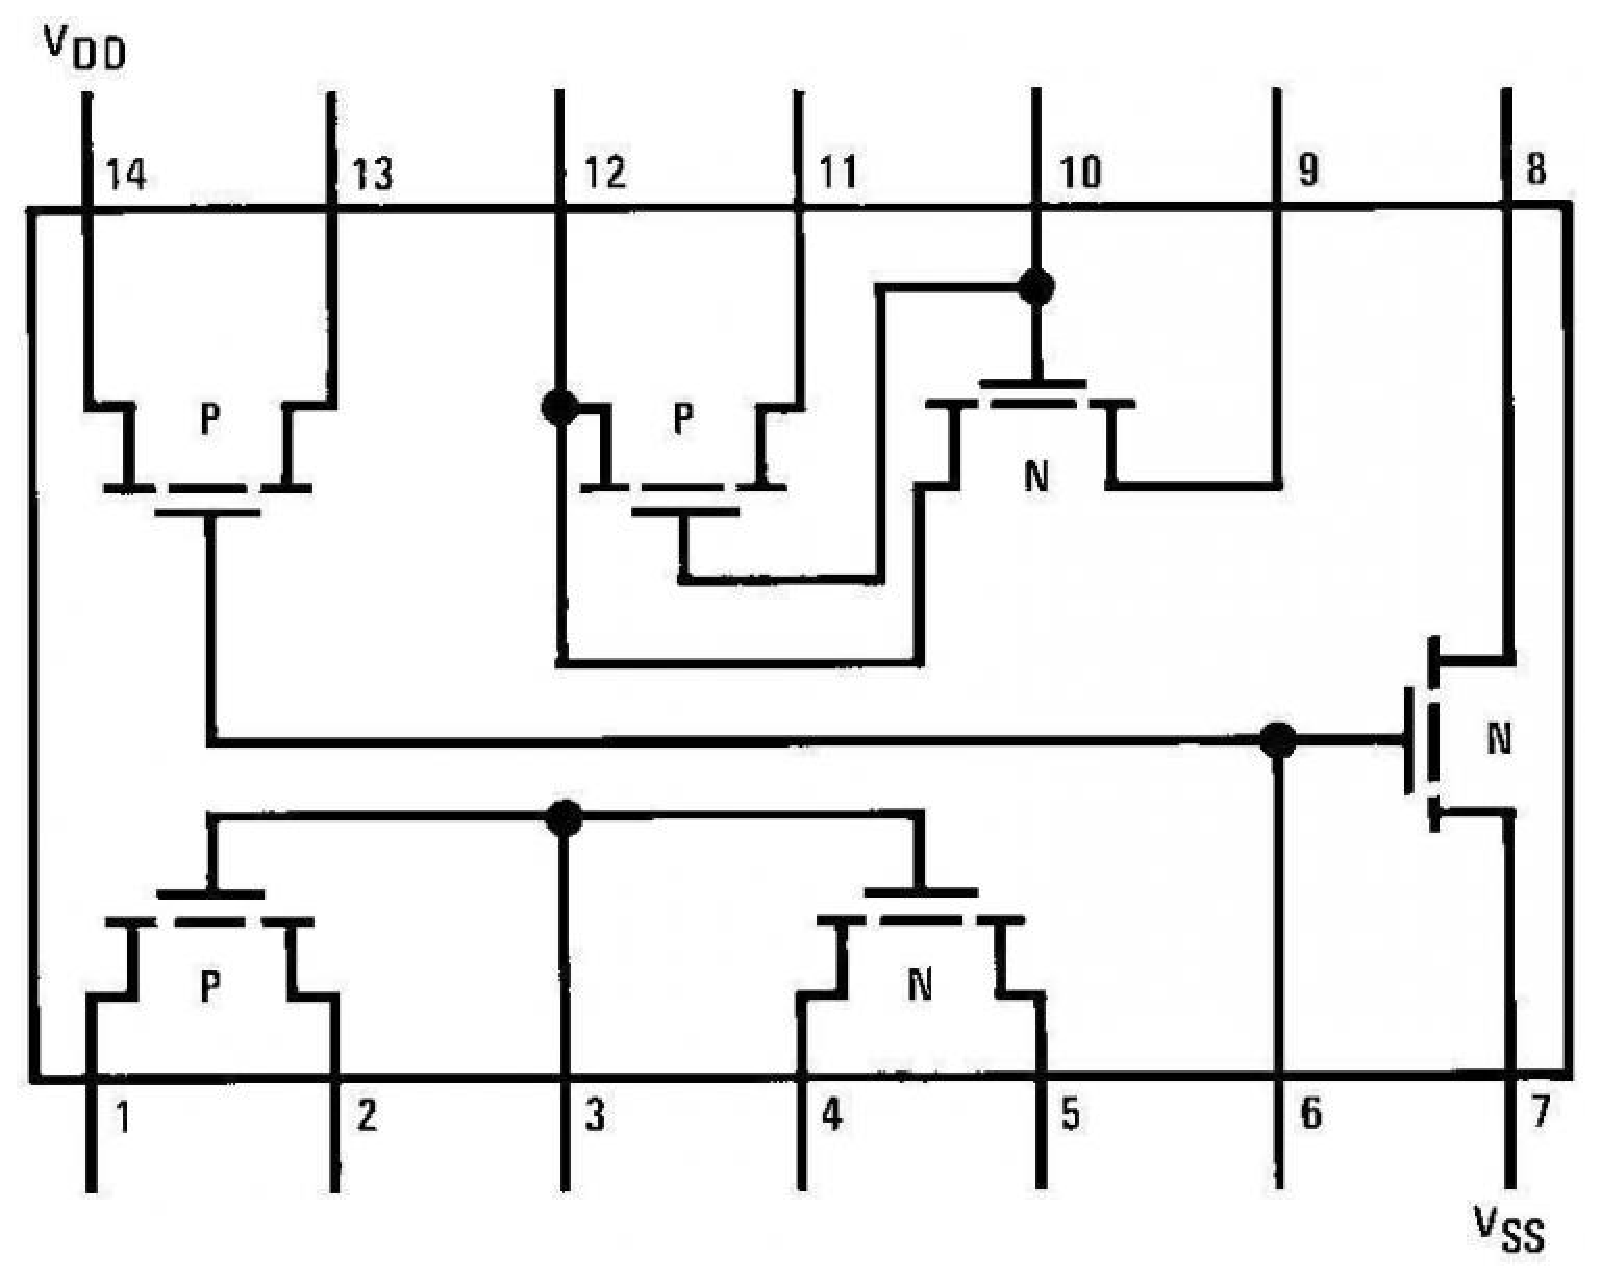
\includegraphics[width=\columnwidth]{./figs/CD4007.eps}} 
 \caption{CD4007}
 \label{fig:exm} 
\end{figure}

\subsection{NOT}
As shown in Fig. \ref{fig:not}, one PMOS and one NMOS elements in Fig. \ref{fig:exm} are required.


\begin{figure}[!h]
\centering
\resizebox {\columnwidth} {!} {
\begin{circuitikz}[american voltages, european resistors]
\draw
  (0,0) node[pmos] (pmosA) {}
  (0,-2) node[nmos] (nmosB) {}
  (pmosA.G) to (nmosB.G)
  (pmosA.D) to (nmosB.D)
  ($(pmosA.G)!0.5!(nmosB.G)$) to[short,-o] ++(-1,0) node[left] {W}
  ($(pmosA.D)!0.5!(nmosB.D)$) to[short,-o] ++(1,0) node[right] {$\overline{W}$}
  (nmosB.S) node[ground] {}
  (pmosA.S) to[short,-o] ++(0,0.5) node[left] {VCC};
  
\end{circuitikz}
}
\caption{NOT Gate}
\label{fig:not}
\end{figure}

\subsection{NAND}
 
NAND gate is one of the two universal logic gates which can be used to construct any logic gate.
Fig. \ref{fig:NAND-2} shows how to construct a 2 input NAND gate.
\begin{figure}[!h]
\centering
\resizebox {\columnwidth} {!} {
\begin{circuitikz}[american voltages, european resistors]
\draw
(0,0) node[pmos] (pmosA) {}
(2,0) node[pmos] (pmosB) {}
(pmosA.S) to (pmosB.S)
($(pmosA.S)!0.5!(pmosB.S)$) to [short,*-o] ++(0,1) {} node[right] {VCC}
(pmosA.D) to (pmosB.D)
($(pmosA.D)!0.5!(pmosB.D)$) to [short,-*]  ++(0,0) node[nmos,anchor=D] (nmosD) {}
(1,-3) node[nmos] (nmosE) {}
(nmosD.S) to (nmosE.D)
(nmosE.S) node[ground] {}
(pmosA.G) to[short,-o] ++(0,0) node[left] {A}
(pmosB.G) to[short,-o] ++(0,0) node[left] {B}
(nmosD.G) to[short,-o] ++(0,0) node[left] {A}
(nmosE.G) to[short,-o] ++(0,0) node[left] {B}
(pmosA.D) to (pmosB.D) 
 to [short,*-o] ++(1,0) {} node[right] {$Y=\overline{AB}$};

\end{circuitikz}

}
\caption{2 - Input NAND Gate}
\label{fig:NAND-2}
\end{figure}
%
3-input NAND gate can be formed with the help of CMOS as per Fig. \ref{fig:NAND-3}.
%
\begin{figure}[!h]
\centering
\resizebox {\columnwidth} {!} {
\begin{circuitikz}[american voltages, european resistors]
\draw
(0,0) node[pmos] (pmosA) {}
(2,0) node[pmos] (pmosB) {}
(4,0) node[pmos] (pmosC) {}
(pmosA.S) to (pmosB.S) to (pmosC.S)
($(pmosA.S)!0.5!(pmosB.S)$) to [short,*-o] ++(0,1) {} node[right] {VCC}
(pmosA.D) to (pmosB.D) to (pmosC.D)
($(pmosA.D)!0.5!(pmosB.D)$) to [short,-*]  ++(0,0) node[nmos,anchor=D] (nmosD) {}
(1,-3) node[nmos] (nmosE) {}
(1,-4.5) node[nmos] (nmosF) {}
(nmosD.S) to (nmosE.D)
(nmosE.S) to (nmosF.D)
(nmosF.S) node[ground] {}
(pmosA.G) to[short,-o] ++(0,0) node[left] {A}
(pmosB.G) to[short,-o] ++(0,0) node[left] {B}
(pmosC.G) to[short,-o] ++(0,0) node[left] {C}
(nmosD.G) to[short,-o] ++(0,0) node[left] {A}
(nmosE.G) to[short,-o] ++(0,0) node[left] {B}
(nmosF.G) to[short,-o] ++(0,0) node[left] {C}
(pmosA.D) to (pmosB.D) to (pmosC.D)
 to [short,*-o] ++(1,0) {} node[right] {$Y=\overline{ABC}$};

\end{circuitikz}

}
\caption{3 - Input NAND Gate}
\label{fig:NAND-3}
\end{figure}

\section{Seven Segment Display}
\begin{problem}
Connect the 7447 IC in Fig. \ref{fig:7447}  to the seven segment display in Fig. \ref{fig:sevenseg} and display all numbers from 0-9.
\end{problem}
%
\subsection{Counting Decoder}
%
A counting decoder increments the input by 1 and has the following logic
\begin{align}
\label{eq:countingA}
A&=\overline{W}
\\
B&=W\bar{X}\bar{Z}+\bar{W}X 
\\
C&=\bar{X}Y+\bar{W}Y+WX\bar{Y}
\\
D&=\bar{W}Z+WXY
\label{eq:countingD}
\end{align}
\begin{center}
\end{center}
where W,X,Y,Z are inputs and A,B,C,D are outputs.
%
\begin{figure}[!h]
\centering
\resizebox {\columnwidth} {!} {
%\documentclass{standalone}
%\usepackage{tikz}
%\usepackage{amsmath,amssymb}
%\makeatletter
%\newsavebox\myboxA
%\newsavebox\myboxB
%\newlength\mylenA
%\newcommand*\xoverline[2][0.75]{%
%    \sbox{\myboxA}{$\m@th#2$}%
%    \setbox\myboxB\null% Phantom box
%    \ht\myboxB=\ht\myboxA%
%    \dp\myboxB=\dp\myboxA%
%    \wd\myboxB=#1\wd\myboxA% Scale phantom
%    \sbox\myboxB{$\m@th\overline{\copy\myboxB}$}%  Overlined phantom
%    \setlength\mylenA{\the\wd\myboxA}%   calc width diff
%    \addtolength\mylenA{-\the\wd\myboxB}%
%    \ifdim\wd\myboxB<\wd\myboxA%
%       \rlap{\hskip 0.5\mylenA\usebox\myboxB}{\usebox\myboxA}%
%    \else
%        \hskip -0.5\mylenA\rlap{\usebox\myboxA}{\hskip 0.5\mylenA\usebox\myboxB}%
%    \fi}
%\makeatother
%
%
%\begin{document}

\begin{tikzpicture}[scale=1,
     pin/.style={draw,rectangle,minimum width=2em,font=\small}
     ]
%   \clip (18,.5) rectangle (5,2);           
%Vertices of the main display rectangle
\def \xmin{0}
\def \xmax{17}
\def \ymin{0}
\def \ymax{6}

%Number of pins on a side
\def \n{8}
\def \k{1.6}

%Draw the display rectangle


%Define height of pins and their separation
\def \height{2}
\pgfmathsetmacro{\centx}{(\xmax+\xmin)/2}
\pgfmathsetmacro{\centy}{(\ymax+\ymin)/2}
\pgfmathsetmacro{\wid}{(\xmax-\xmin)/(\n-1)}


\draw ({\xmin-0.5*\wid},\ymin)rectangle ({\xmax+0.5*\wid},\ymax);

%Defining y axis divisions
\pgfmathsetmacro{\ywid}{(\ymin-\ymax)/(\n-2)}

%Putting text 7447 at the centre
   \node at (\centx,\centy) {\textbf{\LARGE{7447}}};

      
\foreach [count=\i] \k in {$V_{CC}$,$\bar{f}$,$\bar{g}$,$\bar{a}$,$\bar{b}$,$\bar{c}$,$\bar{d}$,$\bar{e}$}
   {
\pgfmathsetmacro{\j}{int(round(17-\i)}
\draw node[pin,anchor=center] at ({\xmin+(\i-1)*\wid},{\ymin-0.15*\wid}){\LARGE \i};
\draw node[pin,anchor=center] at ({\xmin+(\i-1)*\wid},{\ymax+0.15*\wid}){\LARGE \j};
            \node (\i) at ( {\xmin+(\i-1)*\wid},{\ymax+0.45*\wid}) {\LARGE \k} ;
   }

\foreach [count=\i] \k in {$B$,$C$,,,,$D$,$A$,GND}
{
            \node (\i) at ( {\xmin+(\i-1)*\wid},{\ymin-0.45*\wid}) {\LARGE \k} ;              
 }
\draw (-0.5*\wid,{\centy-0.5}) arc (-90:90:0.5) ;
 \end{tikzpicture}
%\end{document}
}
\caption{7447}
\label{fig:7447}
\end{figure}
%
%
\begin{figure}[!h]
\centering
\resizebox {\columnwidth} {!} {
%\subsection{Introduction}
\renewcommand{\theequation}{\theenumi}
\renewcommand{\thefigure}{\theenumi}
\begin{enumerate}[label=\thesection.\arabic*.,ref=\thesection.\theenumi]
\numberwithin{equation}{enumi}
\numberwithin{figure}{enumi}
\numberwithin{table}{enumi}

\item  Fig. \ref{fig:sevenseg} shows a seven segment display with pins $a,b,c,d,e,f,g$.  Each of these pins is connected to an LED (light emitting device).

\begin{figure}[!ht]
\centering
\resizebox {\columnwidth} {!} {
%\subsection{Introduction}
\renewcommand{\theequation}{\theenumi}
\renewcommand{\thefigure}{\theenumi}
\begin{enumerate}[label=\thesection.\arabic*.,ref=\thesection.\theenumi]
\numberwithin{equation}{enumi}
\numberwithin{figure}{enumi}
\numberwithin{table}{enumi}

\item  Fig. \ref{fig:sevenseg} shows a seven segment display with pins $a,b,c,d,e,f,g$.  Each of these pins is connected to an LED (light emitting device).

\begin{figure}[!ht]
\centering
\resizebox {\columnwidth} {!} {
%\subsection{Introduction}
\renewcommand{\theequation}{\theenumi}
\renewcommand{\thefigure}{\theenumi}
\begin{enumerate}[label=\thesection.\arabic*.,ref=\thesection.\theenumi]
\numberwithin{equation}{enumi}
\numberwithin{figure}{enumi}
\numberwithin{table}{enumi}

\item  Fig. \ref{fig:sevenseg} shows a seven segment display with pins $a,b,c,d,e,f,g$.  Each of these pins is connected to an LED (light emitting device).

\begin{figure}[!ht]
\centering
\resizebox {\columnwidth} {!} {
\input{./figs/sevenseg.tex}
}
\caption{}
\label{fig:sevenseg}
\end{figure}

\item Fig. \ref{fig:sevenseg12} shows how to generate the numbers on the display using Table
\ref{table:arduioport}.  Complete Table \ref{table:arduioport} by drawing the figures for all numbers from 0-9.

\begin{figure}[!h]
\begin{center}
\resizebox {\columnwidth} {!} {
\input{./figs/sevenseg12.tex}
}
\end{center}
\caption{}
\label{fig:sevenseg12}
\end{figure}


\begin{table}[!h]
\centering
\input{./tables/arduinoport.tex}
\caption{}
\label{table:arduioport}
\end{table}


\end{enumerate}

}
\caption{}
\label{fig:sevenseg}
\end{figure}

\item Fig. \ref{fig:sevenseg12} shows how to generate the numbers on the display using Table
\ref{table:arduioport}.  Complete Table \ref{table:arduioport} by drawing the figures for all numbers from 0-9.

\begin{figure}[!h]
\begin{center}
\resizebox {\columnwidth} {!} {
%
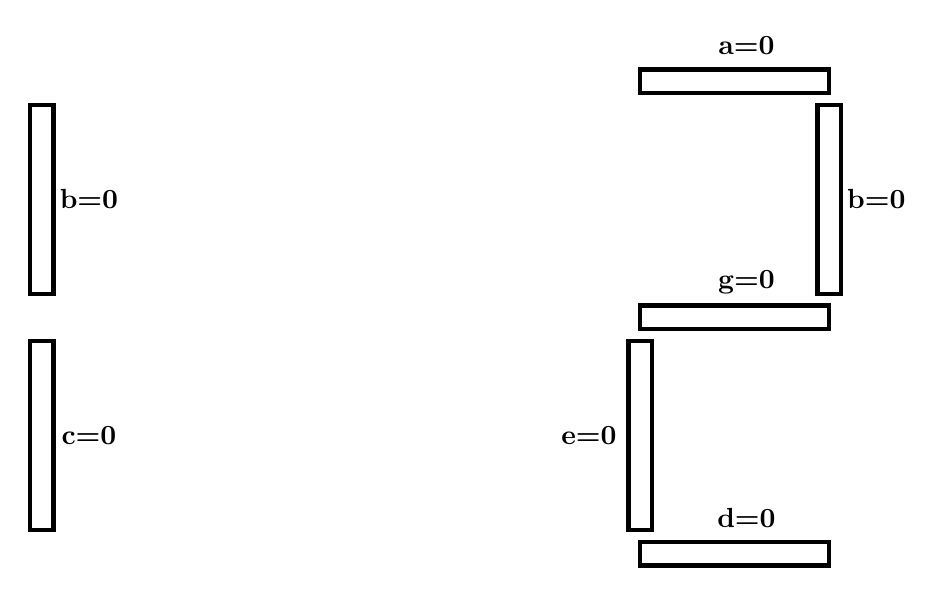
\begin{tikzpicture}
  [
    scale=1,
    >=stealth,
    point/.style = {draw, circle,  fill = black, inner sep = 0.5pt},
    dot/.style   = {draw, circle,  fill = black, inner sep = .2pt},
  ]

%Vertices of the main display rectangle
\def \xmin{0}
\def \xmax{6}
\def \ymin{0}
\def \ymax{-9}

%Number of pins on a side
\def \n{5}
\def \k{1.6}

%Define height of pins and their separation
\def \height{2}
\pgfmathsetmacro{\wid}{(\xmax-\xmin)/(\n-1)}

%Defining y axis divisions
\pgfmathsetmacro{\ywid}{(\ymin-\ymax)/(\n-2)}

%Drawing 1
\foreach [count=\i] \j in {\textbf{b=0},\textbf{c=0}}
{            
\draw[ultra thick] (\xmin+2.6*\wid,{\ymin-(\i+0.35)*\ywid } ) rectangle +(0.3,\k*\wid );
\node (\i) at ( \xmin + 3.1*\wid,{\ymin-(\i-0.05)*\ywid}) {\j} ;
}

%Drawing 2, scope helps create another figure by reusing the same coordinates
\begin{scope}[shift={(10,0)}]
\foreach [count=\i] \j in {\textbf{a=0},\textbf{g=0},\textbf{d=0}}
{            
\draw[ultra thick] (\xmin+1.1*\wid,{\ymin-(\i-0.5)*\ywid} ) rectangle +(\k*\wid,0.3 );
\node (\i) at ( \xmin + 2*\wid,{\ymin-(\i-0.7)*\ywid}) {\j} ;
}

\foreach [count=\i] \j in {\textbf{f},\textbf{e=0}}
{
\ifnum \i=2
            
\draw[ultra thick] (\xmin+\wid,{\ymin-(\i+0.35)*\ywid} ) rectangle +(0.3,\k*\wid );

\node (\i) at ( \xmin + \wid-0.5,{\ymin-(\i-0.05)*\ywid}) {\j} ;
\fi
}

\foreach [count=\i] \j in {\textbf{b=0},\textbf{c}}
{  
\ifnum \i = 1          
\draw[ultra thick] (\xmin+2.6*\wid,{\ymin-(\i+0.35)*\ywid } ) rectangle +(0.3,\k*\wid );
\node (\i) at ( \xmin + 3.1*\wid,{\ymin-(\i-0.05)*\ywid}) {\j} ;
\fi
}
  \end{scope}

%
\end{tikzpicture}

}
\end{center}
\caption{}
\label{fig:sevenseg12}
\end{figure}


\begin{table}[!h]
\centering
%%%%%%%%%%%%%%%%%%%%%%%%%%%%%%%%%%%%%%%%%%%%%%%%%%%%%%%%%%%%%%%%%%%%%%
%%                                                                  %%
%%  This is the header of a LaTeX2e file exported from Gnumeric.    %%
%%                                                                  %%
%%  This file can be compiled as it stands or included in another   %%
%%  LaTeX document. The table is based on the longtable package so  %%
%%  the longtable options (headers, footers...) can be set in the   %%
%%  preamble section below (see PRAMBLE).                           %%
%%                                                                  %%
%%  To include the file in another, the following two lines must be %%
%%  in the including file:                                          %%
%%        \def\inputGnumericTable{}                                 %%
%%  at the beginning of the file and:                               %%
%%        \input{name-of-this-file.tex}                             %%
%%  where the table is to be placed. Note also that the including   %%
%%  file must use the following packages for the table to be        %%
%%  rendered correctly:                                             %%
%%    \usepackage[latin1]{inputenc}                                 %%
%%    \usepackage{color}                                            %%
%%    \usepackage{array}                                            %%
%%    \usepackage{longtable}                                        %%
%%    \usepackage{calc}                                             %%
%%    \usepackage{multirow}                                         %%
%%    \usepackage{hhline}                                           %%
%%    \usepackage{ifthen}                                           %%
%%  optionally (for landscape tables embedded in another document): %%
%%    \usepackage{lscape}                                           %%
%%                                                                  %%
%%%%%%%%%%%%%%%%%%%%%%%%%%%%%%%%%%%%%%%%%%%%%%%%%%%%%%%%%%%%%%%%%%%%%%



%%  This section checks if we are begin input into another file or  %%
%%  the file will be compiled alone. First use a macro taken from   %%
%%  the TeXbook ex 7.7 (suggestion of Han-Wen Nienhuys).            %%
\def\ifundefined#1{\expandafter\ifx\csname#1\endcsname\relax}


%%  Check for the \def token for inputed files. If it is not        %%
%%  defined, the file will be processed as a standalone and the     %%
%%  preamble will be used.                                          %%
\ifundefined{inputGnumericTable}

%%  We must be able to close or not the document at the end.        %%
	\def\gnumericTableEnd{\end{document}}


%%%%%%%%%%%%%%%%%%%%%%%%%%%%%%%%%%%%%%%%%%%%%%%%%%%%%%%%%%%%%%%%%%%%%%
%%                                                                  %%
%%  This is the PREAMBLE. Change these values to get the right      %%
%%  paper size and other niceties.                                  %%
%%                                                                  %%
%%%%%%%%%%%%%%%%%%%%%%%%%%%%%%%%%%%%%%%%%%%%%%%%%%%%%%%%%%%%%%%%%%%%%%

	\documentclass[12pt%
			  %,landscape%
                    ]{report}
       \usepackage[latin1]{inputenc}
       \usepackage{fullpage}
       \usepackage{color}
       \usepackage{array}
       \usepackage{longtable}
       \usepackage{calc}
       \usepackage{multirow}
       \usepackage{hhline}
       \usepackage{ifthen}

	\begin{document}


%%  End of the preamble for the standalone. The next section is for %%
%%  documents which are included into other LaTeX2e files.          %%
\else

%%  We are not a stand alone document. For a regular table, we will %%
%%  have no preamble and only define the closing to mean nothing.   %%
    \def\gnumericTableEnd{}

%%  If we want landscape mode in an embedded document, comment out  %%
%%  the line above and uncomment the two below. The table will      %%
%%  begin on a new page and run in landscape mode.                  %%
%       \def\gnumericTableEnd{\end{landscape}}
%       \begin{landscape}


%%  End of the else clause for this file being \input.              %%
\fi

%%%%%%%%%%%%%%%%%%%%%%%%%%%%%%%%%%%%%%%%%%%%%%%%%%%%%%%%%%%%%%%%%%%%%%
%%                                                                  %%
%%  The rest is the gnumeric table, except for the closing          %%
%%  statement. Changes below will alter the table's appearance.     %%
%%                                                                  %%
%%%%%%%%%%%%%%%%%%%%%%%%%%%%%%%%%%%%%%%%%%%%%%%%%%%%%%%%%%%%%%%%%%%%%%

\providecommand{\gnumericmathit}[1]{#1} 
%%  Uncomment the next line if you would like your numbers to be in %%
%%  italics if they are italizised in the gnumeric table.           %%
%\renewcommand{\gnumericmathit}[1]{\mathit{#1}}
\providecommand{\gnumericPB}[1]%
{\let\gnumericTemp=\\#1\let\\=\gnumericTemp\hspace{0pt}}
 \ifundefined{gnumericTableWidthDefined}
        \newlength{\gnumericTableWidth}
        \newlength{\gnumericTableWidthComplete}
        \newlength{\gnumericMultiRowLength}
        \global\def\gnumericTableWidthDefined{}
 \fi
%% The following setting protects this code from babel shorthands.  %%
 \ifthenelse{\isundefined{\languageshorthands}}{}{\languageshorthands{english}}
%%  The default table format retains the relative column widths of  %%
%%  gnumeric. They can easily be changed to c, r or l. In that case %%
%%  you may want to comment out the next line and uncomment the one %%
%%  thereafter                                                      %%
\providecommand\gnumbox{\makebox[0pt]}
%%\providecommand\gnumbox[1][]{\makebox}

%% to adjust positions in multirow situations                       %%
\setlength{\bigstrutjot}{\jot}
\setlength{\extrarowheight}{\doublerulesep}

%%  The \setlongtables command keeps column widths the same across  %%
%%  pages. Simply comment out next line for varying column widths.  %%
\setlongtables

\setlength\gnumericTableWidth{%
	10pt+%
	10pt+%
	10pt+%
	10pt+%
	10pt+%
	10pt+%
	10pt+%
	30pt+%
0pt}
\def\gumericNumCols{8}
\setlength\gnumericTableWidthComplete{\gnumericTableWidth+%
         \tabcolsep*\gumericNumCols*2+\arrayrulewidth*\gumericNumCols}
\ifthenelse{\lengthtest{\gnumericTableWidthComplete > \linewidth}}%
         {\def\gnumericScale{\ratio{\linewidth-%
                        \tabcolsep*\gumericNumCols*2-%
                        \arrayrulewidth*\gumericNumCols}%
{\gnumericTableWidth}}}%
{\def\gnumericScale{1}}

%%%%%%%%%%%%%%%%%%%%%%%%%%%%%%%%%%%%%%%%%%%%%%%%%%%%%%%%%%%%%%%%%%%%%%
%%                                                                  %%
%% The following are the widths of the various columns. We are      %%
%% defining them here because then they are easier to change.       %%
%% Depending on the cell formats we may use them more than once.    %%
%%                                                                  %%
%%%%%%%%%%%%%%%%%%%%%%%%%%%%%%%%%%%%%%%%%%%%%%%%%%%%%%%%%%%%%%%%%%%%%%

\ifthenelse{\isundefined{\gnumericColA}}{\newlength{\gnumericColA}}{}\settowidth{\gnumericColA}{\begin{tabular}{@{}p{10pt*\gnumericScale}@{}}x\end{tabular}}
\ifthenelse{\isundefined{\gnumericColB}}{\newlength{\gnumericColB}}{}\settowidth{\gnumericColB}{\begin{tabular}{@{}p{10pt*\gnumericScale}@{}}x\end{tabular}}
\ifthenelse{\isundefined{\gnumericColC}}{\newlength{\gnumericColC}}{}\settowidth{\gnumericColC}{\begin{tabular}{@{}p{10pt*\gnumericScale}@{}}x\end{tabular}}
\ifthenelse{\isundefined{\gnumericColD}}{\newlength{\gnumericColD}}{}\settowidth{\gnumericColD}{\begin{tabular}{@{}p{10pt*\gnumericScale}@{}}x\end{tabular}}
\ifthenelse{\isundefined{\gnumericColE}}{\newlength{\gnumericColE}}{}\settowidth{\gnumericColE}{\begin{tabular}{@{}p{10pt*\gnumericScale}@{}}x\end{tabular}}
\ifthenelse{\isundefined{\gnumericColF}}{\newlength{\gnumericColF}}{}\settowidth{\gnumericColF}{\begin{tabular}{@{}p{10pt*\gnumericScale}@{}}x\end{tabular}}
\ifthenelse{\isundefined{\gnumericColG}}{\newlength{\gnumericColG}}{}\settowidth{\gnumericColG}{\begin{tabular}{@{}p{10pt*\gnumericScale}@{}}x\end{tabular}}
\ifthenelse{\isundefined{\gnumericColH}}{\newlength{\gnumericColH}}{}\settowidth{\gnumericColH}{\begin{tabular}{@{}p{30pt*\gnumericScale}@{}}x\end{tabular}}

%\resizebox{\columnwidth}{!}
%{
\begin{tabular}{
%\begin{longtable}[c]{%
	b{\gnumericColA}%
	b{\gnumericColB}%
	b{\gnumericColC}%
	b{\gnumericColD}%
	b{\gnumericColE}%
	b{\gnumericColF}%
	b{\gnumericColG}%
	b{\gnumericColH}%
	}

%%%%%%%%%%%%%%%%%%%%%%%%%%%%%%%%%%%%%%%%%%%%%%%%%%%%%%%%%%%%%%%%%%%%%%
%%  The longtable options. (Caption, headers... see Goosens, p.124) %%
%	\caption{The Table Caption.}             \\	%
% \hline	% Across the top of the table.
%%  The rest of these options are table rows which are placed on    %%
%%  the first, last or every page. Use \multicolumn if you want.    %%

%%  Header for the first page.                                      %%
%	\multicolumn{8}{c}{The First Header} \\ \hline 
%	\multicolumn{1}{c}{colTag}	%Column 1
%	&\multicolumn{1}{c}{colTag}	%Column 2
%	&\multicolumn{1}{c}{colTag}	%Column 3
%	&\multicolumn{1}{c}{colTag}	%Column 4
%	&\multicolumn{1}{c}{colTag}	%Column 5
%	&\multicolumn{1}{c}{colTag}	%Column 6
%	&\multicolumn{1}{c}{colTag}	%Column 7
%	&\multicolumn{1}{c}{colTag}	\\ \hline %Last column
%	\endfirsthead

%%  The running header definition.                                  %%
%	\hline
%	\multicolumn{8}{l}{\ldots\small\slshape continued} \\ \hline
%	\multicolumn{1}{c}{colTag}	%Column 1
%	&\multicolumn{1}{c}{colTag}	%Column 2
%	&\multicolumn{1}{c}{colTag}	%Column 3
%	&\multicolumn{1}{c}{colTag}	%Column 4
%	&\multicolumn{1}{c}{colTag}	%Column 5
%	&\multicolumn{1}{c}{colTag}	%Column 6
%	&\multicolumn{1}{c}{colTag}	%Column 7
%	&\multicolumn{1}{c}{colTag}	\\ \hline %Last column
%	\endhead

%%  The running footer definition.                                  %%
%	\hline
%	\multicolumn{8}{r}{\small\slshape continued\ldots} \\
%	\endfoot

%%  The ending footer definition.                                   %%
%	\multicolumn{8}{c}{That's all folks} \\ \hline 
%	\endlastfoot
%%%%%%%%%%%%%%%%%%%%%%%%%%%%%%%%%%%%%%%%%%%%%%%%%%%%%%%%%%%%%%%%%%%%%%

\hhline{|-|-|-|-|-|-|-|-}
	 \multicolumn{1}{|p{\gnumericColA}|}%
	{\gnumericPB{\centering}\gnumbox{a}}
	&\multicolumn{1}{p{\gnumericColB}|}%
	{\gnumericPB{\centering}\gnumbox{b}}
	&\multicolumn{1}{p{\gnumericColC}|}%
	{\gnumericPB{\centering}\gnumbox{c}}
	&\multicolumn{1}{p{\gnumericColD}|}%
	{\gnumericPB{\centering}\gnumbox{d}}
	&\multicolumn{1}{p{\gnumericColE}|}%
	{\gnumericPB{\centering}\gnumbox{e}}
	&\multicolumn{1}{p{\gnumericColF}|}%
	{\gnumericPB{\centering}\gnumbox{f}}
	&\multicolumn{1}{p{\gnumericColG}|}%
	{\gnumericPB{\centering}\gnumbox{g}}
	&\multicolumn{1}{p{\gnumericColH}|}%
	{\gnumericPB{\centering}\gnumbox{decimal}}
\\
\hhline{|--------|}
	 \multicolumn{1}{|p{\gnumericColA}|}%
	{\gnumericPB{\centering}\gnumbox{1}}
	&\multicolumn{1}{p{\gnumericColB}|}%
	{\gnumericPB{\centering}\gnumbox{0}}
	&\multicolumn{1}{p{\gnumericColC}|}%
	{\gnumericPB{\centering}\gnumbox{0}}
	&\multicolumn{1}{p{\gnumericColD}|}%
	{\gnumericPB{\centering}\gnumbox{1}}
	&\multicolumn{1}{p{\gnumericColE}|}%
	{\gnumericPB{\centering}\gnumbox{1}}
	&\multicolumn{1}{p{\gnumericColF}|}%
	{\gnumericPB{\centering}\gnumbox{1}}
	&\multicolumn{1}{p{\gnumericColG}|}%
	{\gnumericPB{\centering}\gnumbox{1}}
	&\multicolumn{1}{p{\gnumericColH}|}%
	{\gnumericPB{\centering}\gnumbox{1}}
\\
\hhline{|--------|}
	 \multicolumn{1}{|p{\gnumericColA}|}%
	{\gnumericPB{\centering}\gnumbox{0}}
	&\multicolumn{1}{p{\gnumericColB}|}%
	{\gnumericPB{\centering}\gnumbox{0}}
	&\multicolumn{1}{p{\gnumericColC}|}%
	{\gnumericPB{\centering}\gnumbox{1}}
	&\multicolumn{1}{p{\gnumericColD}|}%
	{\gnumericPB{\centering}\gnumbox{0}}
	&\multicolumn{1}{p{\gnumericColE}|}%
	{\gnumericPB{\centering}\gnumbox{0}}
	&\multicolumn{1}{p{\gnumericColF}|}%
	{\gnumericPB{\centering}\gnumbox{1}}
	&\multicolumn{1}{p{\gnumericColG}|}%
	{\gnumericPB{\centering}\gnumbox{0}}
	&\multicolumn{1}{p{\gnumericColH}|}%
	{\gnumericPB{\centering}\gnumbox{2}}
\\
\hhline{|-|-|-|-|-|-|-|-|}
%\end{longtable}
\end{tabular}
%}
\ifthenelse{\isundefined{\languageshorthands}}{}{\languageshorthands{\languagename}}
\gnumericTableEnd

\caption{}
\label{table:arduioport}
\end{table}


\end{enumerate}

}
\caption{}
\label{fig:sevenseg}
\end{figure}

\item Fig. \ref{fig:sevenseg12} shows how to generate the numbers on the display using Table
\ref{table:arduioport}.  Complete Table \ref{table:arduioport} by drawing the figures for all numbers from 0-9.

\begin{figure}[!h]
\begin{center}
\resizebox {\columnwidth} {!} {
%
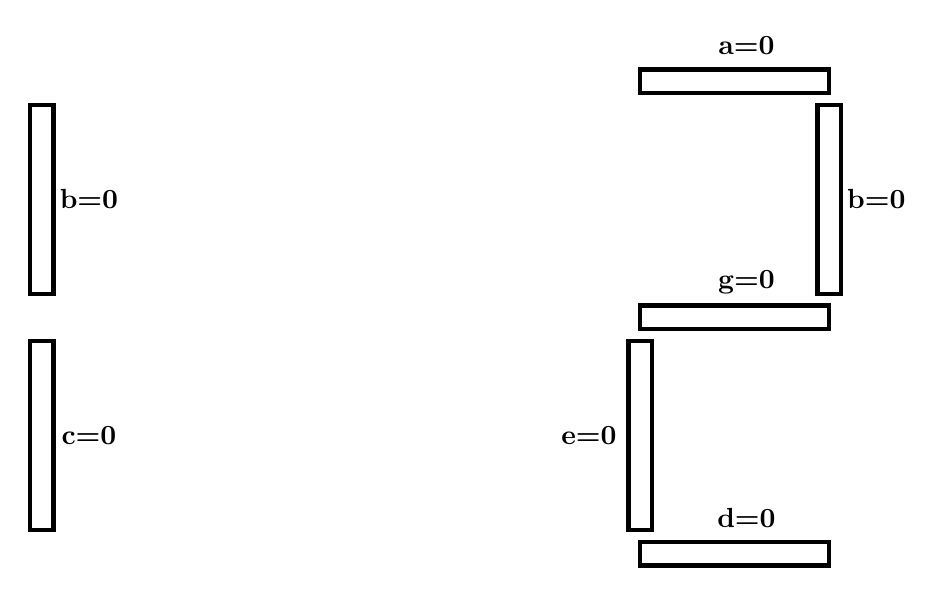
\begin{tikzpicture}
  [
    scale=1,
    >=stealth,
    point/.style = {draw, circle,  fill = black, inner sep = 0.5pt},
    dot/.style   = {draw, circle,  fill = black, inner sep = .2pt},
  ]

%Vertices of the main display rectangle
\def \xmin{0}
\def \xmax{6}
\def \ymin{0}
\def \ymax{-9}

%Number of pins on a side
\def \n{5}
\def \k{1.6}

%Define height of pins and their separation
\def \height{2}
\pgfmathsetmacro{\wid}{(\xmax-\xmin)/(\n-1)}

%Defining y axis divisions
\pgfmathsetmacro{\ywid}{(\ymin-\ymax)/(\n-2)}

%Drawing 1
\foreach [count=\i] \j in {\textbf{b=0},\textbf{c=0}}
{            
\draw[ultra thick] (\xmin+2.6*\wid,{\ymin-(\i+0.35)*\ywid } ) rectangle +(0.3,\k*\wid );
\node (\i) at ( \xmin + 3.1*\wid,{\ymin-(\i-0.05)*\ywid}) {\j} ;
}

%Drawing 2, scope helps create another figure by reusing the same coordinates
\begin{scope}[shift={(10,0)}]
\foreach [count=\i] \j in {\textbf{a=0},\textbf{g=0},\textbf{d=0}}
{            
\draw[ultra thick] (\xmin+1.1*\wid,{\ymin-(\i-0.5)*\ywid} ) rectangle +(\k*\wid,0.3 );
\node (\i) at ( \xmin + 2*\wid,{\ymin-(\i-0.7)*\ywid}) {\j} ;
}

\foreach [count=\i] \j in {\textbf{f},\textbf{e=0}}
{
\ifnum \i=2
            
\draw[ultra thick] (\xmin+\wid,{\ymin-(\i+0.35)*\ywid} ) rectangle +(0.3,\k*\wid );

\node (\i) at ( \xmin + \wid-0.5,{\ymin-(\i-0.05)*\ywid}) {\j} ;
\fi
}

\foreach [count=\i] \j in {\textbf{b=0},\textbf{c}}
{  
\ifnum \i = 1          
\draw[ultra thick] (\xmin+2.6*\wid,{\ymin-(\i+0.35)*\ywid } ) rectangle +(0.3,\k*\wid );
\node (\i) at ( \xmin + 3.1*\wid,{\ymin-(\i-0.05)*\ywid}) {\j} ;
\fi
}
  \end{scope}

%
\end{tikzpicture}

}
\end{center}
\caption{}
\label{fig:sevenseg12}
\end{figure}


\begin{table}[!h]
\centering
%%%%%%%%%%%%%%%%%%%%%%%%%%%%%%%%%%%%%%%%%%%%%%%%%%%%%%%%%%%%%%%%%%%%%%
%%                                                                  %%
%%  This is the header of a LaTeX2e file exported from Gnumeric.    %%
%%                                                                  %%
%%  This file can be compiled as it stands or included in another   %%
%%  LaTeX document. The table is based on the longtable package so  %%
%%  the longtable options (headers, footers...) can be set in the   %%
%%  preamble section below (see PRAMBLE).                           %%
%%                                                                  %%
%%  To include the file in another, the following two lines must be %%
%%  in the including file:                                          %%
%%        \def\inputGnumericTable{}                                 %%
%%  at the beginning of the file and:                               %%
%%        \input{name-of-this-file.tex}                             %%
%%  where the table is to be placed. Note also that the including   %%
%%  file must use the following packages for the table to be        %%
%%  rendered correctly:                                             %%
%%    \usepackage[latin1]{inputenc}                                 %%
%%    \usepackage{color}                                            %%
%%    \usepackage{array}                                            %%
%%    \usepackage{longtable}                                        %%
%%    \usepackage{calc}                                             %%
%%    \usepackage{multirow}                                         %%
%%    \usepackage{hhline}                                           %%
%%    \usepackage{ifthen}                                           %%
%%  optionally (for landscape tables embedded in another document): %%
%%    \usepackage{lscape}                                           %%
%%                                                                  %%
%%%%%%%%%%%%%%%%%%%%%%%%%%%%%%%%%%%%%%%%%%%%%%%%%%%%%%%%%%%%%%%%%%%%%%



%%  This section checks if we are begin input into another file or  %%
%%  the file will be compiled alone. First use a macro taken from   %%
%%  the TeXbook ex 7.7 (suggestion of Han-Wen Nienhuys).            %%
\def\ifundefined#1{\expandafter\ifx\csname#1\endcsname\relax}


%%  Check for the \def token for inputed files. If it is not        %%
%%  defined, the file will be processed as a standalone and the     %%
%%  preamble will be used.                                          %%
\ifundefined{inputGnumericTable}

%%  We must be able to close or not the document at the end.        %%
	\def\gnumericTableEnd{\end{document}}


%%%%%%%%%%%%%%%%%%%%%%%%%%%%%%%%%%%%%%%%%%%%%%%%%%%%%%%%%%%%%%%%%%%%%%
%%                                                                  %%
%%  This is the PREAMBLE. Change these values to get the right      %%
%%  paper size and other niceties.                                  %%
%%                                                                  %%
%%%%%%%%%%%%%%%%%%%%%%%%%%%%%%%%%%%%%%%%%%%%%%%%%%%%%%%%%%%%%%%%%%%%%%

	\documentclass[12pt%
			  %,landscape%
                    ]{report}
       \usepackage[latin1]{inputenc}
       \usepackage{fullpage}
       \usepackage{color}
       \usepackage{array}
       \usepackage{longtable}
       \usepackage{calc}
       \usepackage{multirow}
       \usepackage{hhline}
       \usepackage{ifthen}

	\begin{document}


%%  End of the preamble for the standalone. The next section is for %%
%%  documents which are included into other LaTeX2e files.          %%
\else

%%  We are not a stand alone document. For a regular table, we will %%
%%  have no preamble and only define the closing to mean nothing.   %%
    \def\gnumericTableEnd{}

%%  If we want landscape mode in an embedded document, comment out  %%
%%  the line above and uncomment the two below. The table will      %%
%%  begin on a new page and run in landscape mode.                  %%
%       \def\gnumericTableEnd{\end{landscape}}
%       \begin{landscape}


%%  End of the else clause for this file being \input.              %%
\fi

%%%%%%%%%%%%%%%%%%%%%%%%%%%%%%%%%%%%%%%%%%%%%%%%%%%%%%%%%%%%%%%%%%%%%%
%%                                                                  %%
%%  The rest is the gnumeric table, except for the closing          %%
%%  statement. Changes below will alter the table's appearance.     %%
%%                                                                  %%
%%%%%%%%%%%%%%%%%%%%%%%%%%%%%%%%%%%%%%%%%%%%%%%%%%%%%%%%%%%%%%%%%%%%%%

\providecommand{\gnumericmathit}[1]{#1} 
%%  Uncomment the next line if you would like your numbers to be in %%
%%  italics if they are italizised in the gnumeric table.           %%
%\renewcommand{\gnumericmathit}[1]{\mathit{#1}}
\providecommand{\gnumericPB}[1]%
{\let\gnumericTemp=\\#1\let\\=\gnumericTemp\hspace{0pt}}
 \ifundefined{gnumericTableWidthDefined}
        \newlength{\gnumericTableWidth}
        \newlength{\gnumericTableWidthComplete}
        \newlength{\gnumericMultiRowLength}
        \global\def\gnumericTableWidthDefined{}
 \fi
%% The following setting protects this code from babel shorthands.  %%
 \ifthenelse{\isundefined{\languageshorthands}}{}{\languageshorthands{english}}
%%  The default table format retains the relative column widths of  %%
%%  gnumeric. They can easily be changed to c, r or l. In that case %%
%%  you may want to comment out the next line and uncomment the one %%
%%  thereafter                                                      %%
\providecommand\gnumbox{\makebox[0pt]}
%%\providecommand\gnumbox[1][]{\makebox}

%% to adjust positions in multirow situations                       %%
\setlength{\bigstrutjot}{\jot}
\setlength{\extrarowheight}{\doublerulesep}

%%  The \setlongtables command keeps column widths the same across  %%
%%  pages. Simply comment out next line for varying column widths.  %%
\setlongtables

\setlength\gnumericTableWidth{%
	10pt+%
	10pt+%
	10pt+%
	10pt+%
	10pt+%
	10pt+%
	10pt+%
	30pt+%
0pt}
\def\gumericNumCols{8}
\setlength\gnumericTableWidthComplete{\gnumericTableWidth+%
         \tabcolsep*\gumericNumCols*2+\arrayrulewidth*\gumericNumCols}
\ifthenelse{\lengthtest{\gnumericTableWidthComplete > \linewidth}}%
         {\def\gnumericScale{\ratio{\linewidth-%
                        \tabcolsep*\gumericNumCols*2-%
                        \arrayrulewidth*\gumericNumCols}%
{\gnumericTableWidth}}}%
{\def\gnumericScale{1}}

%%%%%%%%%%%%%%%%%%%%%%%%%%%%%%%%%%%%%%%%%%%%%%%%%%%%%%%%%%%%%%%%%%%%%%
%%                                                                  %%
%% The following are the widths of the various columns. We are      %%
%% defining them here because then they are easier to change.       %%
%% Depending on the cell formats we may use them more than once.    %%
%%                                                                  %%
%%%%%%%%%%%%%%%%%%%%%%%%%%%%%%%%%%%%%%%%%%%%%%%%%%%%%%%%%%%%%%%%%%%%%%

\ifthenelse{\isundefined{\gnumericColA}}{\newlength{\gnumericColA}}{}\settowidth{\gnumericColA}{\begin{tabular}{@{}p{10pt*\gnumericScale}@{}}x\end{tabular}}
\ifthenelse{\isundefined{\gnumericColB}}{\newlength{\gnumericColB}}{}\settowidth{\gnumericColB}{\begin{tabular}{@{}p{10pt*\gnumericScale}@{}}x\end{tabular}}
\ifthenelse{\isundefined{\gnumericColC}}{\newlength{\gnumericColC}}{}\settowidth{\gnumericColC}{\begin{tabular}{@{}p{10pt*\gnumericScale}@{}}x\end{tabular}}
\ifthenelse{\isundefined{\gnumericColD}}{\newlength{\gnumericColD}}{}\settowidth{\gnumericColD}{\begin{tabular}{@{}p{10pt*\gnumericScale}@{}}x\end{tabular}}
\ifthenelse{\isundefined{\gnumericColE}}{\newlength{\gnumericColE}}{}\settowidth{\gnumericColE}{\begin{tabular}{@{}p{10pt*\gnumericScale}@{}}x\end{tabular}}
\ifthenelse{\isundefined{\gnumericColF}}{\newlength{\gnumericColF}}{}\settowidth{\gnumericColF}{\begin{tabular}{@{}p{10pt*\gnumericScale}@{}}x\end{tabular}}
\ifthenelse{\isundefined{\gnumericColG}}{\newlength{\gnumericColG}}{}\settowidth{\gnumericColG}{\begin{tabular}{@{}p{10pt*\gnumericScale}@{}}x\end{tabular}}
\ifthenelse{\isundefined{\gnumericColH}}{\newlength{\gnumericColH}}{}\settowidth{\gnumericColH}{\begin{tabular}{@{}p{30pt*\gnumericScale}@{}}x\end{tabular}}

%\resizebox{\columnwidth}{!}
%{
\begin{tabular}{
%\begin{longtable}[c]{%
	b{\gnumericColA}%
	b{\gnumericColB}%
	b{\gnumericColC}%
	b{\gnumericColD}%
	b{\gnumericColE}%
	b{\gnumericColF}%
	b{\gnumericColG}%
	b{\gnumericColH}%
	}

%%%%%%%%%%%%%%%%%%%%%%%%%%%%%%%%%%%%%%%%%%%%%%%%%%%%%%%%%%%%%%%%%%%%%%
%%  The longtable options. (Caption, headers... see Goosens, p.124) %%
%	\caption{The Table Caption.}             \\	%
% \hline	% Across the top of the table.
%%  The rest of these options are table rows which are placed on    %%
%%  the first, last or every page. Use \multicolumn if you want.    %%

%%  Header for the first page.                                      %%
%	\multicolumn{8}{c}{The First Header} \\ \hline 
%	\multicolumn{1}{c}{colTag}	%Column 1
%	&\multicolumn{1}{c}{colTag}	%Column 2
%	&\multicolumn{1}{c}{colTag}	%Column 3
%	&\multicolumn{1}{c}{colTag}	%Column 4
%	&\multicolumn{1}{c}{colTag}	%Column 5
%	&\multicolumn{1}{c}{colTag}	%Column 6
%	&\multicolumn{1}{c}{colTag}	%Column 7
%	&\multicolumn{1}{c}{colTag}	\\ \hline %Last column
%	\endfirsthead

%%  The running header definition.                                  %%
%	\hline
%	\multicolumn{8}{l}{\ldots\small\slshape continued} \\ \hline
%	\multicolumn{1}{c}{colTag}	%Column 1
%	&\multicolumn{1}{c}{colTag}	%Column 2
%	&\multicolumn{1}{c}{colTag}	%Column 3
%	&\multicolumn{1}{c}{colTag}	%Column 4
%	&\multicolumn{1}{c}{colTag}	%Column 5
%	&\multicolumn{1}{c}{colTag}	%Column 6
%	&\multicolumn{1}{c}{colTag}	%Column 7
%	&\multicolumn{1}{c}{colTag}	\\ \hline %Last column
%	\endhead

%%  The running footer definition.                                  %%
%	\hline
%	\multicolumn{8}{r}{\small\slshape continued\ldots} \\
%	\endfoot

%%  The ending footer definition.                                   %%
%	\multicolumn{8}{c}{That's all folks} \\ \hline 
%	\endlastfoot
%%%%%%%%%%%%%%%%%%%%%%%%%%%%%%%%%%%%%%%%%%%%%%%%%%%%%%%%%%%%%%%%%%%%%%

\hhline{|-|-|-|-|-|-|-|-}
	 \multicolumn{1}{|p{\gnumericColA}|}%
	{\gnumericPB{\centering}\gnumbox{a}}
	&\multicolumn{1}{p{\gnumericColB}|}%
	{\gnumericPB{\centering}\gnumbox{b}}
	&\multicolumn{1}{p{\gnumericColC}|}%
	{\gnumericPB{\centering}\gnumbox{c}}
	&\multicolumn{1}{p{\gnumericColD}|}%
	{\gnumericPB{\centering}\gnumbox{d}}
	&\multicolumn{1}{p{\gnumericColE}|}%
	{\gnumericPB{\centering}\gnumbox{e}}
	&\multicolumn{1}{p{\gnumericColF}|}%
	{\gnumericPB{\centering}\gnumbox{f}}
	&\multicolumn{1}{p{\gnumericColG}|}%
	{\gnumericPB{\centering}\gnumbox{g}}
	&\multicolumn{1}{p{\gnumericColH}|}%
	{\gnumericPB{\centering}\gnumbox{decimal}}
\\
\hhline{|--------|}
	 \multicolumn{1}{|p{\gnumericColA}|}%
	{\gnumericPB{\centering}\gnumbox{1}}
	&\multicolumn{1}{p{\gnumericColB}|}%
	{\gnumericPB{\centering}\gnumbox{0}}
	&\multicolumn{1}{p{\gnumericColC}|}%
	{\gnumericPB{\centering}\gnumbox{0}}
	&\multicolumn{1}{p{\gnumericColD}|}%
	{\gnumericPB{\centering}\gnumbox{1}}
	&\multicolumn{1}{p{\gnumericColE}|}%
	{\gnumericPB{\centering}\gnumbox{1}}
	&\multicolumn{1}{p{\gnumericColF}|}%
	{\gnumericPB{\centering}\gnumbox{1}}
	&\multicolumn{1}{p{\gnumericColG}|}%
	{\gnumericPB{\centering}\gnumbox{1}}
	&\multicolumn{1}{p{\gnumericColH}|}%
	{\gnumericPB{\centering}\gnumbox{1}}
\\
\hhline{|--------|}
	 \multicolumn{1}{|p{\gnumericColA}|}%
	{\gnumericPB{\centering}\gnumbox{0}}
	&\multicolumn{1}{p{\gnumericColB}|}%
	{\gnumericPB{\centering}\gnumbox{0}}
	&\multicolumn{1}{p{\gnumericColC}|}%
	{\gnumericPB{\centering}\gnumbox{1}}
	&\multicolumn{1}{p{\gnumericColD}|}%
	{\gnumericPB{\centering}\gnumbox{0}}
	&\multicolumn{1}{p{\gnumericColE}|}%
	{\gnumericPB{\centering}\gnumbox{0}}
	&\multicolumn{1}{p{\gnumericColF}|}%
	{\gnumericPB{\centering}\gnumbox{1}}
	&\multicolumn{1}{p{\gnumericColG}|}%
	{\gnumericPB{\centering}\gnumbox{0}}
	&\multicolumn{1}{p{\gnumericColH}|}%
	{\gnumericPB{\centering}\gnumbox{2}}
\\
\hhline{|-|-|-|-|-|-|-|-|}
%\end{longtable}
\end{tabular}
%}
\ifthenelse{\isundefined{\languageshorthands}}{}{\languageshorthands{\languagename}}
\gnumericTableEnd

\caption{}
\label{table:arduioport}
\end{table}


\end{enumerate}

}
\caption{Seven Segment Display}
\label{fig:sevenseg}
\end{figure}
%
\subsection{CMOS Counting Decoder}
\begin{problem}
Express \eqref{eq:countingA}-\eqref{eq:countingD} using NAND logic
\end{problem}
\solution
\begin{align}
A&=\overline{W}
\\
B&=W\bar{X}\bar{Z}+\bar{W}X =\overline{(\overline{W\bar{X}\bar{Z}}).(\overline{\bar{W}X})}
\\
C&=\bar{X}Y+\bar{W}Y+WX\bar{Y}
\\
&=\overline{(\overline{\bar{X}Y}).(\overline{\bar{W}Y}).(\overline{WX\bar{Y}})}
\\
D&=\bar{W}Z+WXY=\overline{(\overline{\bar{W}Z}).(\overline{WXY})}
\end{align}
\begin{problem}
Express $A$ through CMOS logic.
\end{problem}
\solution
The logic for A is an inverter. Construct a circuit similar to Fig.\ref{fig:not} which is a simple NOT gate.
When input is W then output is $\overline{W}$.
\begin{problem}
Express $B$ through CMOS logic.
\end{problem}
\solution Fig. \ref{fig:CMOS_B}, followed by Fig. \ref{fig:not}.
\begin{figure}[!h]
\centering
\resizebox {\columnwidth} {!} {
\begin{tikzpicture}
    \node (x) at (0, 2) {$W$};
    \node (y) at (-1, 1) {$\bar{X}$};
    \node (z) at (0.5, 0) {$\bar{Z}$};

    
    \node[nand gate US, draw, rotate=0, logic gate inputs=nnn] at ($(y) + (2, 0.085)$) (xory) {};

    \draw (x) -- ([xshift=0.2cm]x) |-(xory.input 1);
    \draw (y) -- ([xshift=0.2cm]y) |-(xory.input 2);
    \draw (z) -| ($(y) + (1.2, -0.2)$) |- (xory.input 3);


    
        
   
   
      
    \node (x) at (0, -2) {$\bar{W}$};
    \node (y) at (-0.5, -3) {$X$};
        
    \node[nand gate US, draw, rotate=0, logic gate inputs=nn] at ($(y) + (2, 0.085)$) (xory1) {};

    \draw (x) -- ([xshift=0.2cm]x) |-(xory1.input 1);
    \draw (y) -- ([xshift=0.2cm]y) |-(xory1.input 2);
         
     \node[nand gate US, draw, rotate=0, logic gate inputs=nn] at ($(xory.output) + (2, -2)$) (xory2) {};

    \draw (xory.output) -- ([xshift=0.2cm]xory.output) |-(xory2.input 1);
    \draw (xory1.output) -- ([xshift=0.2cm]xory1.output) |-(xory2.input 2);
     \draw (xory2.output) -- node[above]{$W\bar{X}\bar{Z}+\bar{W}X $} ($(xory2) + (3, 0)$);
      

\end{tikzpicture}

}
\caption{CMOS Logic for $\overline{B}$}
\label{fig:CMOS_B}
\end{figure}
\begin{problem}
Express $C$ through CMOS logic.
\end{problem}
\solution Fig. \ref{fig:CMOS_C}, followed by Fig. \ref{fig:not}.
\begin{figure}[!h]
\centering
\resizebox {\columnwidth} {!} {
\begin{tikzpicture}
    \node (x) at (0.5, 2) {$\bar{X}$};
    \node (y) at (0, 1) {$Y$};
    
    
    \node[nand gate US, draw, rotate=0, logic gate inputs=nn] at ($(y) + (2, 0.085)$) (xory) {};
     \draw (x) -- ([xshift=0.2cm]x) |- (xory.input 1);
    \draw (y) -- ([xshift=0.2cm]y) |-(xory.input 2);
    
    \node (x) at (0.5, -1) {$\bar{W}$};
    \node (y) at (0, -2) {$Y$};
    
    
    \node[nand gate US, draw, rotate=0, logic gate inputs=nn] at ($(y) + (2, 0.085)$) (xory1) {};
    \draw (x) -- ([xshift=0.2cm]x) |-(xory1.input 1);
    \draw (y) -- ([xshift=1cm]y) |-(xory1.input 2);
    
      
    \node (x) at (0.5, -4) {$W$};
    \node (y) at (0, -5) {$X$};
    \node (z) at (0.7, -6) {$\bar{Y}$};

    
    \node[nand gate US, draw, rotate=0, logic gate inputs=nnn] at ($(y) + (2, 0.085)$) (xory3) {};
    \draw (x) -- ([xshift=0.2cm]x) |-(xory3.input 1);
    \draw (y) -- ([xshift=0.4cm]y) |-(xory3.input 2);
    \draw (z) -| ($(y) + (0.4, -0.3)$) |- (xory3.input 3);
   
    
    \node[nand gate US, draw, rotate=0, logic gate inputs=nnn] at ($(xory1.output) + (2, 0)$) (xory4) {};

    \draw (xory.output) -- ([xshift=0.2cm]xory.output) |-(xory4.input 1);
    \draw (xory1.output) -- ([xshift=0.2cm]xory1.output) |-(xory4.input 2);
    \draw (xory3.output) -- ([xshift=0.2cm]xory3.output) |-(xory4.input 3);

     \draw (xory4.output) -- node[above]{$\bar{X}Y+\bar{W}Y+WX\bar{Y}$} ($(xory4) + (4, 0)$);
\end{tikzpicture}

}
\caption{CMOS Logic for $\overline{C}$}
\label{fig:CMOS_C}
\end{figure}
\begin{problem}
Express $C$ through CMOS logic.
\end{problem}
\solution Fig. \ref{fig:CMOS_D}, followed by Fig. \ref{fig:not}.

\begin{figure}[!h]
\centering
\resizebox {\columnwidth} {!} {
\begin{tikzpicture}
    \node (x) at (0.5, 2) {${W}$};
    \node (y) at (0, 1) {${X}$};
    \node (z) at (1,0) {${Y}$};

    
    \node[nand gate US, draw, rotate=0, logic gate inputs=nnn] at ($(y) + (2, 0.085)$) (xory) {};

    \draw (x) -- ([xshift=0.2cm]x) |-(xory.input 1);
    \draw (y) -- ([xshift=0.4cm]y) |-(xory.input 2);
    \draw (z) -| ($(y) + (0.6, -0.3)$) |- (xory.input 3);


    
        
   
   
      
     \node (x) at (0.5, -2) {$\bar{W}$};
    \node (y) at (0, -3) {$Z$};
        
    \node[nand gate US, draw, rotate=0, logic gate inputs=nn] at ($(y) + (2, 0.085)$) (xory1) {};

    \draw (x) -- ([xshift=0.2cm]x) |-(xory1.input 1);
    \draw (y) -- ([xshift=0.2cm]y) |-(xory1.input 2);
         
     \node[nand gate US, draw, rotate=0, logic gate inputs=nn] at ($(xory.output) + (2, -2)$) (xory2) {};

    \draw (xory.output) -- ([xshift=0.2cm]xory.output) |-(xory2.input 1);
    \draw (xory1.output) -- ([xshift=0.2cm]xory1.output) |-(xory2.input 2);
     \draw (xory2.output) -- node[above]{$\bar{W}Z+WXY$} ($(xory2) + (3, 0)$);


\end{tikzpicture}

}
\caption{CMOS Logic for $\overline{D}$}
\label{fig:CMOS_D}
\end{figure}

\begin{problem}
Design the 7447 IC using CMOS logic.
\end{problem}
\section{Decade Counter}
%
\subsection{Clock}
Fig. \ref{fig:clock} shows a clock, which is a series of pulses with period $T$.
%
\begin{figure}[!h]
\centering
\resizebox {\columnwidth} {!} {
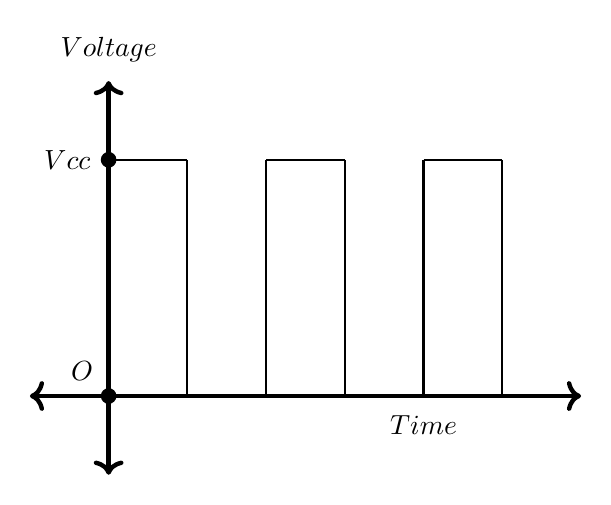
\begin{tikzpicture}
\draw[ultra thick,->](0,0) -- (0,4);
\draw[ultra thick,->](0,0) -- (6,0);
\draw[ultra thick,->](0,0) -- (0,-1);
\draw[ultra thick,->](0,0) -- (-1,0);
\draw[thick](0,3) -- (1,3);
\draw[thick](1,3) -- (1,0);
\draw[thick](2,0) -- (2,3);
\draw[thick](2,3) -- (3,3);
\draw[thick](3,3) -- (3,0);
\draw[thick](4,0) -- (4,3);
\draw[thick](4,3) -- (5,3);
\draw[thick](5,3) -- (5,0);
\node[label={180:{$Vcc$}},circle,fill,inner sep=2pt] at (0,3) {};
\node[label={135:{$O$}},circle,fill,inner sep=2pt] at (0,0) {};
\node[label={90:{$Voltage$}}] at (0,4) {};
\node[label={270:{$Time$}}] at (4,0) {};
\end{tikzpicture}
}
\caption{clock output}
\label{fig:clock}
\end{figure}
\begin{problem}
Design a circuit for generating Fig. \ref{fig:clock}.
\end{problem}
\solution Fig. \ref{fig:clock_circuit} can be used to generate the clock in Fig. \ref{fig:clock}.
\begin{figure}[!h]
\centering
\resizebox {\columnwidth} {!} {
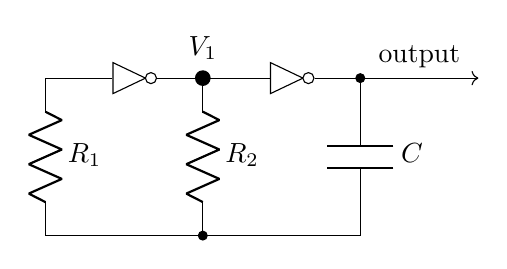
\begin{tikzpicture}
  \node[not gate US, draw] at (1,0) (notx) {};
  \node[not gate US, draw] at (3,0) (noty) {};
  \draw (notx.output) -- (noty.input);
  \draw (0,0) -- (notx.input);
  \draw (noty.output) -- (4,0);
  \draw(0,0) to [R,l=$R_{1}$,-](0,-2);
  \draw(0,-2) -- (4,-2);
  \draw(2,0) to [R,l=$R_{2}$,*-*](2,-2);
   \draw(4,0) to [C,l=$C$,*-](4,-2);
   \draw[->](4,0) -- node[above]{output} (5.5,0);
   
   \node[label={90:{$V_1$}},circle,fill,inner sep=2pt] at (2,0) {};
   
\end{tikzpicture}

}
\caption{Clock Circuit}
\label{fig:clock_circuit}
\end{figure}
%
\begin{problem}
Explain the circuit in Fig. \ref{fig:clock_circuit}.
\end{problem}
\solution In Fig. \ref{fig:clock_circuit},  let ${R_1}>{R_2}$.
The circuit is an astable multivibrator. It is made up of two NOT gates. When the output of second not gate is HIGH, the input of second not gate is LOW. The capacitor charges up which changes the output of second not gate from HIGH to LOW. Now we have output of second not gate LOW and its input HIGH. This makes the capacitor to be reverse biased. This is followed by discharging of capacitor. Due to discharging of capacitor, the output of second not gate again becomes HIGH. This process continues and what the observer observes is a series of HIGH and LOW voltages at the output. 
\begin{problem}
Explain why $R_1 > R_2$.
\end{problem}
\solution The CD4007 IC in Fig. \ref{fig:exm} has input switching voltage point at 0.5Vcc. We are using Vcc as 5V. Hence, input voltages ranging from 3.5 to 5 V are recognised as HIGH and voltages from 0 to 1.5 V as LOW for this IC. The voltages in input and output of second not gate can be only 0 or Vcc. 
%The voltage-time graph of the output is shown in Fig.11.
The schematic turns in the other stage when $V_1$ is equal to the half of the power voltage.
When the second gate output flips from 1 to 0, the capacitor is charged to -0.5Vcc (the left plate is negative), so V1 becomes -0.5Vcc and starts to increase because $R_2$ is connected to Vcc.  $R_1$ does not affect the time period at all. It is placed there so that the input current of the inverter does not affect the work of the schematic. That is why it should be much bigger than $R_2$.
\begin{problem}
Obtain the time period of the clock $T$.
\end{problem}
\solution Let $\tau = R_2C$.  Then,
\begin{align}
{V_1} &= Vcc.(1-e^{-\frac{t}{\tau}}) - \frac{Vcc}{2} .e^{-\frac{t}{\tau}}
\\
&= Vcc - \frac{3.Vcc}{2}.e^{-\frac{t}{\tau}}
\end{align}
%
The switching of the schematic will happen when 
%
\begin{align}
V_1 &= \frac{Vcc}{2}
\\ 
\implies  \frac{Vcc}{2} &= Vcc - \frac{3.Vcc}{2}.e^{-\frac{t}{\tau}}
\\
\implies t &= \tau\ln3 = {R_2}C\ln3 
\end{align}
%
%${}$ becomes equal to 0.5Vcc i.e. $$, so:
%$$$$
%$$\Rightarrow \frac{Vcc}{2} = \frac{3.Vcc}{2}.e^{-\frac{t}{\tau}}$$
%$$\Rightarrow \frac{1}{3} = e^{-\frac{t}{\tau}}$$
%$$\Rightarrow 3 = e^{\frac{t}{\tau}}$$
%$$\Rightarrow ln3 = \frac{t}{\tau}$$
%$$= 1.098612289.{R_2}.C$$
This is the half of the period (because the schematic switches exactly on the half of the Vcc), so the period
\begin{equation}
T = 2t = 2\ln3{R_2}C
\end{equation}
%$$$$
%$$\approx 2.2.{R_2}.{C}$$
We can choose a specific value of ${R_2}$ and $C$ to achieve any particular time period for the clock.
%
\subsection{ Flip Flop}
%
\begin{problem}
Design a circuit for the D-Flip Flop.
\end{problem}
\solution See Fig. \ref{fig:dflipflop}.  Note that a clock is necessary for building a Flip Flop.
\begin{figure}[!h]
\centering
\resizebox {\columnwidth} {!} {
\begin{tikzpicture}
    \node (x) at (0, 2) {${D}$};
    
    
    \node[nand gate US, draw, rotate=0, logic gate inputs=nn] at ($(0,1.085) + (2, 0.085)$) (xory1) {};

    \draw (x) -- ([xshift=0.2cm]x) |-(xory1.input 1);
    
        
     
        
    \node[nand gate US, draw, rotate=0, logic gate inputs=nn] at ($(0,-2) + (2, 0.170)$) (xory2) {};
   \draw(xory2.input 2) -- ($(0.085,-2) + (0,0.085)$); 
   \draw($(0.085,-2) + (0,0.085)$) -- (0.085,1.8);   
    
    
    
    \node[nand gate US, draw, rotate=0, logic gate inputs=nn] at (4,1.085) (xory3) {};
    
        
    \node[nand gate US, draw, rotate=0, logic gate inputs=nn] at (4,-1.915) (xory4) {};
     \draw (xory1.input 2) -- ([xshift=-0.2cm]xory1.input 2) |-(xory2.input 1);
     
          \draw (xory3.input 1) -- ([xshift=-0.2cm]xory3.input 1) |-(xory1.output);
          \draw (xory3.input 2) -- (3,1);
          \draw(3,1) -- (3,-1);
          \draw(3,-1) -- (5,-1);
          \draw(5,-1) -- (5,-2);
          \draw (xory4.output) -- node[above]{$\bar{Q}$} ($(xory4) + (2, 0)$);
          \draw (xory3.output) -- node[above]{$Q$} ($(xory3) + (4, 0)$);
          \draw (xory4.input 2) -- (3,-2);

          \draw (3,-2) -- (3,-3);
          \draw(3,-3) -- (7,-3);
          \draw(7,-3) -- (7,1.085);
          \draw (xory2.output) -- (xory4.input 1);
          \draw[thick,->](0.7,0.-0.3) -- (1.5,-0.3);
          \node[above](x) at (0.8,-0.3) {Clock};
\end{tikzpicture}

}
\caption{D Flip-flop}
\label{fig:dflipflop}
\end{figure}
%
\begin{problem}
Design a decade counter.
\end{problem}
\solution See Fig. \ref{fig:decade}
\begin{figure}[!h]
\centering
\resizebox {\columnwidth} {!} {
\tikzstyle{input} = [coordinate]
\tikzstyle{output} = [coordinate]

\begin{tikzpicture}
\tikzstyle{block} = [draw,minimum size=2em]
\node at (0,-1) (input 1) {$$};
\node at (0,-2) (input 2) {$$};
\node at (0,-3) (input 3) {$$};
\node at (0,-4) (input 4) {$$};
\node[block] at (2,-1) (block1) {circuit for logic A};
\node[block] at (2,-2) (block2) {circuit for logic B};
\node[block] at (2,-3) (block3) {circuit for logic C};
\node[block] at (2,-4) (block4) {circuit for logic D};
\node[block] at (6,-1) (block5) {D flip flp};
\node[block] at (6,-2) (block6) {D flip flp};
\node[block] at (6,-3) (block7) {D flip flp}; 
\node[block] at (6,-4) (block8)  {D flip flp};
\draw [->] (block1) -- node[above,name=A] {$A$} (block5);
\draw [->] (block2) -- node[above,name=A] {$B$} (block6);
\draw [->] (block3) -- node[above,name=A] {$C$} (block7);
\draw [->] (block4) -- node[above,name=A] {$D$} (block8);
\node [output, right of=block5] (output 1) {};
\node [output, right of=block6] (output 2) {};
\node [output, right of=block7] (output 3) {};
\node [output, right of=block8] (output 4) {};
\draw[->] (output 1) -- (7.8,-1);
\draw[->] (output 2) -- (8,-2);
\draw[->] (output 3) -- (8.2,-3);
\draw[->] (output 4) -- (8.4,-4);
\draw (7.8,-1) -- (7.8,1);
\draw (8,-2) -- (8,2);
\draw (8.2,-3) -- (8.2,3);
\draw (8.4,-4) -- (8.4,4);
\foreach \Point in {(7.8,-1), (8,-2), (8.2,-3), (8.4,-4)}{
    \node at \Point {\textbullet};
}
\draw (7.8,1) -- (-0.6,1);
\draw (8,2) -- (-0.8,2);
\draw (8.2,3) -- (-1,3);
\draw (8.4,4) -- (-1.2,4);
\draw (-0.6,1) -- (-0.6,-1);
\draw (-0.8,2) -- (-0.8,-2);
\draw (-1,3) -- (-1,-3);
\draw (-1.2,4) -- (-1.2,-4);
\draw[ultra thick,->](7.5,-0.6) -- (7,-0.6);
\draw[ultra thick](7.5,-0.6) -- (7.5,-1.6);
\draw[ultra thick,->](7.5,-1.6) -- (7,-1.6);
\draw[ultra thick](7.5,-1.6) -- (7.5,-2.6);
\draw[ultra thick,->](7.5,-2.6) -- (7,-2.6);
\draw[ultra thick](7.5,-2.6) -- (7.5,-3.6);
\draw[ultra thick,->](7.5,-3.6) -- (7,-3.6);
\draw[ultra thick](7.5,-3.6) -- (7.5,-5.6);
\draw [ultra thick] (7.5,-5.6) -- node[above] {Clock} (9.5,-5.6);
\draw (7.8,-1) -- node[above] { $$} (8.8,-1);
\draw (8,-2) -- node[above] { $$} (8.8,-2);
\draw (8.2,-3) -- node[above] { $$} (8.8,-3);
\draw (8.4,-4) -- node[above] { $$} (8.8,-4);
\draw [->] (8.8,-1) -- node[above] { $A$} (9.5,-1);
\draw [->] (8.8,-2) -- node[above] { $B$} (9.5,-2);
\draw [->] (8.8,-3) -- node[above] { $C$} (9.5,-3);
\draw [->] (8.8,-4) -- node[above] { $D$} (9.5,-4);
\draw [->] (-0.6,-1) -- node[above] {$W$} (block1);
\draw [->] (-0.8,-2) -- node[above] {$X$} (block2);
\draw [->] (-1,-3) -- node[above] {$Y$} (block3);
\draw [->] (-1.2,-4) -- node[above] {$Z$} (block4);
\end{tikzpicture}

}
\caption{circuit for decade counter}
\label{fig:decade}
\end{figure}

\end{document}




